From Figure \ref{Figure_Comparison} it is clear that the optimal solution substantially out-performs both weekly average managers, and the top manager in each gameweek. This is due to the fact that the optimal solution maximizes the points over the entire season, and not only over one particular gameweek. Further, managers that finish top of the gameweek often use a gamechip in order to maximize their weekly score. 

\newpar

\begin{comment}

\end{comment}

There seem to be some positive correlation between the optimal solution and both the weekly top performers as well as the weekly average scores. From table \ref{Figure_Comparison} one can see that the weekly average and the optimal solution have a tendency of moving in the same direction. Hence, when the optimal solution receive a high score, the weekly average have a tendency of doing the same. This might be due to highly selected players performing well in those particular gameweeks. For instance, if a player that has performed well over the entire season receives an abnormal high score during a gameweek, it is anticipated that the weekly average will increase as most managers select this player. Consider Mohamed Salah, who has had an incredible season. At some point he was selected by more than 63\% of the human managers. Thus, when he performs well it is reasonable to assume that both the average and the optimal solution earn numerous points.

\newpar

As stated in chapter \ref{introduction} it is interesting to compare the optimal solution strategy to that of the manager of leads the overall ranking. Figure \ref{Top_Manager} provides a weekly overview of this comparison.

\begin{figure}[H]
\label{fig:Top_Manager}
    \centering
    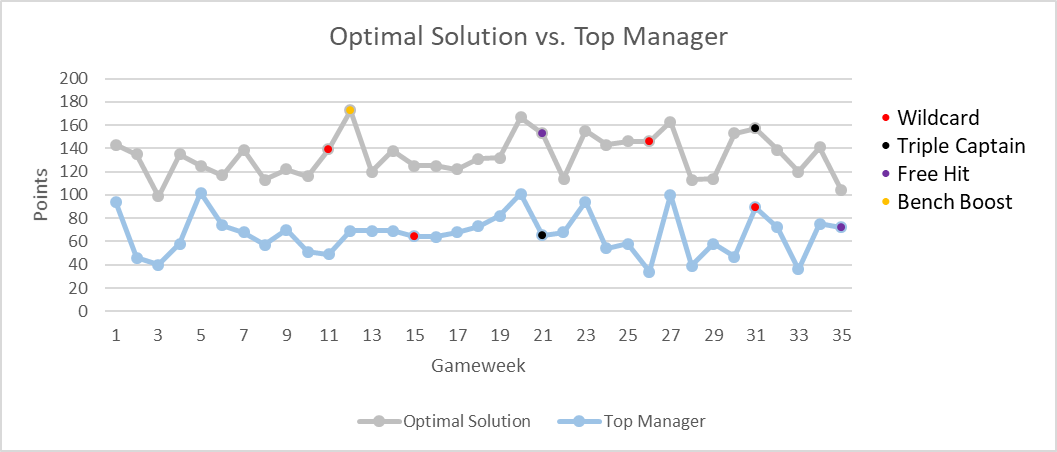
\includegraphics[scale=0.75]{fig/chapter_7/Optimal_vs_Top_colour.png}
    \caption{Comparing optimal solution strategy to top manger}
\label{Top_Manager}    
\end{figure}

As suggested in the introduction, the optimal solution strategy largely outperforms that of the top manager of Fantasy Premier League. In total, it separates 2348 points between the two solutions, more than twice the amount of points gained by the top rated manager. It is notable that the two teams do not play their gamechips in any of the same gameweeks. The top manager played his Triple Captain in gameweek 22, where Tottenham and West Ham were featured twice. Selecting Harry Kane as his Triple Captain is an understandable choice, as Harry Kane was the top scorer of Premier League at that point of time. However, Kane under-performed in both matches only receiving three points in total. In addition, one can see that the top manager played his second Wildcard in gameweek 32, two weeks ahead of a double gameweek. Finally, he played his Free Hit in gameweek 35 which is reasonable as this was ahead of a blank gameweek. As expected, the two teams presented in figure \ref{Top_Manager} are positively correlated.   

\newpar

An interesting comparison is that of the optimal solution to other human managers. Table \ref{Optimal_Human} provides an overview of how the optimal solution strategy performs compared to the top 50\% of the managers. 

\begin{table}[H]
\centering
\caption{Comparing human managers to optimal solution}
\label{Optimal_Human}
\begin{tabular}{llc}
\hline
                 & Mean   & \multicolumn{1}{l}{Percentage of optimal solution} \\
\hline                 
Optimal solution & 133.63 & 100.00 \%                                          \\
Winner           & 66.54  & 49.80 \%                                           \\
Top 5 \%         & 55.83  & 41.78 \%                                           \\
Top 10 \%        & 54.30  & 40.64 \%                                           \\
Top 20 \%        & 52.20  & 39.06 \%                                           \\
Top 30 \%        & 50.40  & 37.72 \%                                           \\
Top 40 \%        & 48.50  & 36.29 \%                                           \\
Top 50 \%        & 46.50  & 34.80 \%                                           \\
\hline
\end{tabular}
\end{table}

As observed, it is an enormous difference between the optimal solution strategy and that of the other human managers. It is remarkable that the difference in mean between the top 50\% and the winner is only slightly above 20 points per round, while the difference between the optimal solution and the winner is above 67 points. Further, it is notable that the difference between finishing in the top 10 percentile to the top 5 percentile is rather low as it only separates 1.43 points per gameweek. In comparison, the difference between the winner and the 5th percentile is as much as 10.71 points per gameweek. Moreover, an interesting point is that this difference is actually larger than the one between the 50th percentile and the 5th percentile. Hence, it provides reason to assume that in order to finish among the absolute best managers, one have to perform extremely well compared to others. 